\documentclass[../main/main.tex]{subfiles}
\begin{document}
%\dominitoc
%\faketableofcontents
\chapter{Contexte cosmologique}\label{cp:cosmo}

\minitoc
\vspace{2cm}
Ce premier chapitre a pour objectif d'introduire les notions
cosmologiques définissant le cadre scientifique dans lequel s'inscrit
cette thèse. 
\newpage
\section{\'Eléments de cosmologie}\label{sec:11}

\subsection{Relativité générale}

Le modèle standard de la cosmologie est basé sur la théorie de la
Relativité Générale d'Einstein
\citep{Einstein1915c,Einstein1915a,Einstein1915b}, permettant de relier la géométrie
de l'espace-temps de l'Univers avec son contenu énergétique. Cette
nouvelle équation de champ s'exprime à travers la relation suivante:

\begin{equation}
  \label{eq:generalrelativity}
  R_{\mu\nu}-\frac{1}{2}Rg_{\mu\nu}+\Lambda g_{\mu\nu}=\frac{8\pi G}{c^{4}}T_{\mu\nu}
\end{equation}
avec:
\begin{itemize}[noitemsep, label=$\diamondsuit$]
\item $R_{\mu\nu}$ le tenseur de Ricci (caractérisant la déformation
  de l'espace-temps);
\item $R$ le scalaire de Ricci (correspondant à la courbure
  scalaire);
\item $g_{\mu\nu}$ la métrique de l'espace-temps;
\item $T_{\mu\nu}$ le tenseur énergie-impulsion;
\item $G$ la constante gravitationnelle;
\item $c$ la célérité de la lumière,
\item $\Lambda$ la constante cosmologique.
\end{itemize}

En définissant le tenseur de courbure de l'espace-temps d'Einstein par:
\begin{equation}
  \label{eq:tenseurspacetime}
  G_{\mu\nu} = R_{\mu\nu} - \frac{1}{2}Rg_{\mu\nu} \ 
\end{equation}
et la constante d'Einstein:
\begin{equation}
  \label{eq:einsteinconstante}
  \kappa = \frac{8\pi G}{c^{4}}
\end{equation}
alors en l'absence de constante cosmologique ($\Lambda=0$)
l'équation~\ref{eq:generalrelativity} devient:
\begin{equation}
  \label{eq:einsteinreduce}
  G_{\mu\nu} = \kappa T_{\mu\nu}
\end{equation}
mettant ainsi en évidence le lien étroit entre la géométrie de
l'espace-temps et son contenu énergétique.
La constante cosmologique $\Lambda$ fut introduite par Einstein dans le
but d'expliquer un Univers statique, conviction qu'il nourissait. Il est
alors possible d'insérer ce terme d'un côté ou de l'autre de l'équation:
\begin{equation}
  \label{eq:einsteinlambda}
  G_{\mu\nu} + \Lambda g_{\mu\nu} = \kappa T_{\mu\nu} \Longleftrightarrow G_{\mu\nu}  = \kappa T_{\mu\nu} - \Lambda g_{\mu\nu}
\end{equation}

Bien que la position de $\Lambda$ ne change rien mathématiquement, cela peut mener à une
interprétation physique bien différente. À gauche la modification agit
directement sur la structure fondamentale de la courbure de l'espace-temps;
à droite, nous pouvons l'interpréter comme une nouvelle source
énergétique. Ce terme fut rapidement abandonné après la découverte de
l'expansion de l'Univers, réfutant l'hypothèse d'un Univers statique
ayant justifiée son introduction initiale.

La découverte de l'accélération de l'expansion de l'Univers
\citep{Riess1998, Perlmutter1999} a conduit à sa réintroduction, en tant
que source énergétique pouvant expliquer ce phénomène observé et mesuré,
pouvant potentiellement correspondre à une énergie du vide, appelée
énergie sombre (\textit{dark energy}).

\subsection{Symétries de l'Univers: le principe cosmologique}

Le principe cosmologique repose sur des hypothèses simplifiant fortement
la résolution des équations d'Einstein. En supposant certaines symétries
de l'Univers pouvant sembler intuitives, il est possible de contraindre la forme de
la métrique de l'espace-temps $g_{\mu\nu}$. Le principe cosmologique
stipule ainsi un Univers homogène et isotrope à grandes échelles.
Bien entendu ces hypothèses ne sont pas valables aux petites échelles,
comme nous le prouvent par exemple les fluctuations de densité au sein
du système solaire ou dans une même galaxie. Mais de la même manière que
nous ne nous intéressons pas aux fluctuations quantiques pour décrire le
mouvement d'une voiture, ce sont seulement les grandes échelles qui nous
intéressent pour décrire la dynamique générale de notre Univers.

Ces deux hypothèses ont été initialement érigées par George Lemaître
en 1927 \citep{Lemaitre1927}.

\subsubsection{Homogénéité de l'Univers}
L'homogénéité aux grandes échelles signifie que l'apparence générale de
l'Univers ne dépend pas de la position de l'observateur: on parle alors
d'invariance par translation.

Cette hypothèse a été vérifiée grâce à de grands relevés de galaxies du
ciel profond, sur des échelles au delà du milliard d'années-lumière
comme par exemple avec le \textit{Sloan Digital Sky Survey}
(SDSS\footnote{\url{https://www.sdss.org}}).
En sondant l'espace à trois dimensions, ces relevés ont montré une
répartition aléatoire des galaxies au delà du milliard d'années-lumière
(voir Figure~\ref{fig:homogenesdss}), témoignant de cette homogénéité spatiale.

\begin{figure}[ht]
  \centering
  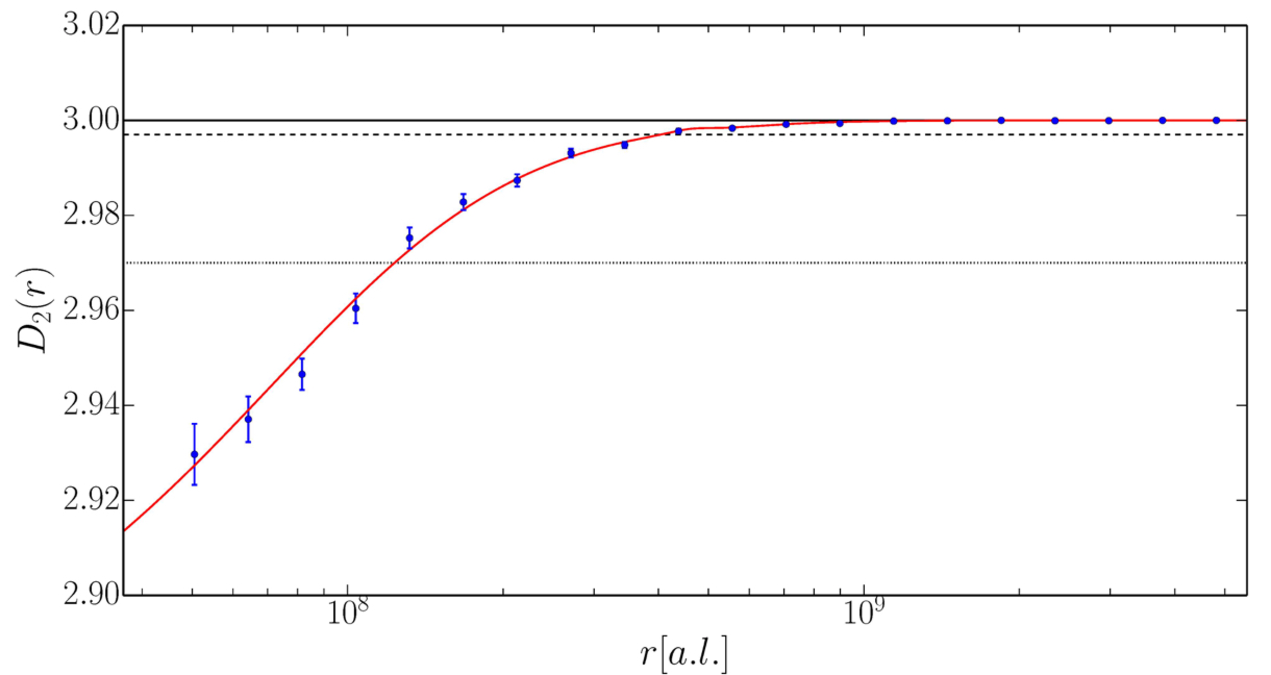
\includegraphics[width=0.75\textwidth]{../figures/01_cosmology/homogeneunivers.pdf}
  \caption[Dimension de corrélation fractale de l’Univers.]{Dimension de
    corrélation fractale de l’Univers sur une échelle de plusieurs
    milliards d'années-lumière. Cette quantité vaut 3 si l’Univers est
    homogène. On voit que c’est le cas à partir d’une échelle d’environ
    $10^{9}$ années-lumière. Figure de \citet{Laurent2016}. Ces
    résultats sont obtenus à partir de spectres de quasars mesurés par
    la collaboration \textit{Baryon Oscillation Spectroscopic Survey} (BOSS) au sein de SDSS.}
\label{fig:homogenesdss}
\end{figure}

\subsubsection{Isotropie de l'Univers}

L'autre hypothèse du principe cosmologique, l'isotropie de l'Univers,
stipule que sa structure est identique quelque soit la direction
d'observation: on parle alors d'invariance par rotation.

L'expérience scientifique la plus connue vérifiant cette caractéristique
est la mesure du fond diffus cosmologique (\textit{Cosmic Wave
  Background}; CMB, aussi appelé rayonnement fossile). Ce signal correspond au plus ancien rayonnement
électromagnétique observable, estimé à $\sim380,000$ ans après le Big
Bang. Avant cela l'Univers était si chaud et dense que les particules
de lumière, les photons, étaient continuellement absorbés, émis et
diffusés par les électrons environnant: le libre parcours moyen des
photons est alors infime, et l'Univers est qualifié \og d'opaque\fg{} pour la
lumière.
Après un refroidissement suffisant de l'Univers ($\sim380,000$ ans après le Big
Bang), les électrons et
les noyaux atomiques se combinent pour former les premiers atomes, c'est
la recombinaison. Les photons circulent alors librement dans l'Univers
qui est devenu \og transparent\fg{}: c'est ce qu'on appelle le découplage et
c'est ce premier rayonnement qui constitue le fond diffus cosmologique.

L'observation de ce fond diffus cosmologique soutient ainsi fortement l'hypothèse
d'isotropie de l'Univers, témoignant d'une intensité similaire dans
toutes les directions, avec une fluctuation de l'ordre de $10^{-5}$
Kelvin.
La Figure~\ref{fig:cmb} présente une carte des anisotropies du fond
diffus cosmologique, basée sur les résultats les plus récents de la
collaboration Planck \citep{Planckisotropy18}.
\begin{figure}[ht]
  \centering
  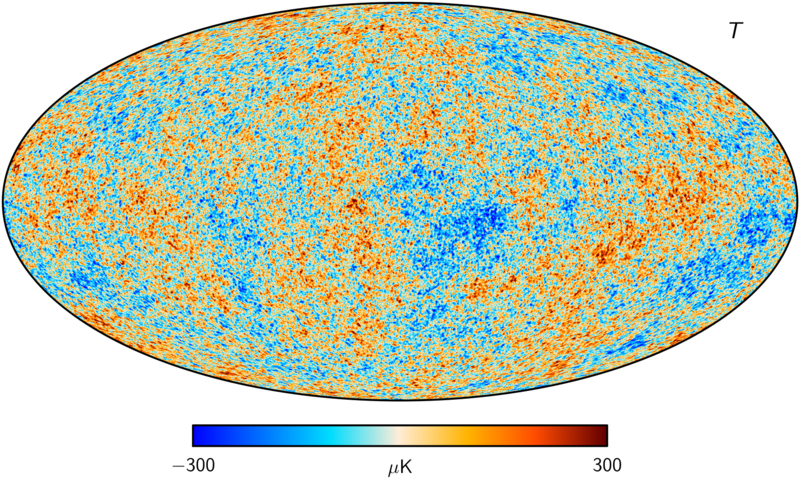
\includegraphics[width=0.9\textwidth]{../figures/01_cosmology/CMB_Planck18.png}
  \caption[Carte des anisotropies de température du fond diffus
  cosmologique (CMB).]{Carte des anisotropies de température du fond
    diffus cosmologique (CMB). Figure basée sur
    \citet{Planckisotropy18}.}
\label{fig:cmb}
\end{figure}

\subsection{Métrique de Friedmann-Lemaître-Robertson-Walker}\label{ssec:FLRW}

Les symétries induites par le principe cosmologique imposent à la partie
spatiale de notre Univers d'avoir la forme d'un espace 3D avec une
courbure constante: un espace Euclidien, une 3-Sphère ou une
3-Hyperboloïde. En prenant en compte l'évolution temporelle de la
géométrie de l'univers (les symétries restent conservées), nous avons de
manière générale la métrique d'espace-temps de Friedmann-Lemaître-Robertson-Walker (FLRW)
\citep{Friedmann1922,Lemaitre1933,Robertson1936,Walker1937}, qui s'écrit
en coordonnées polaires:

\begin{equation}
  \label{eq:FLRW}
  \d s^{2}=c^{2}\d t^{2}-a^{2}(t)\left( \frac{\d r^{2}}{1-kr^{2}}+r^{2}(\d\theta^{2}+\sin^{2}\theta\d\phi^{2})\right)
\end{equation}
où $\d s^{2}$ est un élément infinitésiment d'espace-temps, ($r$,
$\theta$, $\phi$, $t$) les coordonnées d'espace-temps, $a(t)$ le
facteur d'échelle et $k$ un facteur géométrique pouvant prendre les
valeurs ($-1$, $0$, $1$) pour un Univers ouvert, plat ou fermé
respectivement.

Pour ($r$, $\theta$, $\phi$) constants, les objets
suivent l'expansion de l'Univers: ce sont des coordonnées comobiles.
Le facteur d'échelle $a(t)$ est défini comme le rapport entre la
distance séparant deux points immobiles à l'instant $t$ et celle à un
instant de référence $t_{0}$ (normalisé tel que $a(t_{0})=1$). Il trace
ainsi l'influence de l'expansion de l'Univers sur la distance entre deux
points au cours du temps, reliant la distance comobile à la distance
physique.

Il est assez commun de rencontrer la métrique FLRW sous la forme
suivante:
\begin{equation}
  \label{eq:FLRW2}
  \d s^{2}=c^{2}\d t^{2}-a^{2}(t) \left( \d\chi^{2}+S^{2}_{k}(\chi)(\d\theta^{2}+\sin^{2}\theta \d\phi^{2}) \right)
\end{equation}

Avec 
\begin{equation}
  \label{eq:chiflrw}
  S_{k}(\chi) =
  \begin{cases}
        \sin(\chi) & \text{si }  k=1 \\
        \chi & \text{si }  k=0 \\
        \sinh(\chi) & \text{si }  k=-1
    \end{cases}
\end{equation}
et le changement de variable:  $d\chi^{2}=\frac{dr^{2}}{1-kr^{2}}$ $\forall k$.


Les symétries induites par le principe cosmologique vont également
restreindre le tenseur énergie-impulsion $T_{\mu\nu}$ dà celui d'un
fluide parfait (sans transport de chaleur ou de viscosité), s'écrivant
alors sous la forme:
\begin{equation}
  \label{eq:Tmunu}
  T_{\mu\nu} = \left( \rho + \frac{p}{c^{2}}\right)u_{\mu}u_{\nu}+pg_{\mu\nu}
\end{equation}
où $\rho$ et $p$ sont respectivement la densité et la pression du fluide
considéré, et $u_{\mu}$, $u_{\nu}$ les quadri-vitesses du fluide avec la
convention du tenseur métrique $g_{\mu\nu}=\text{diag}(-1,+1,+1,+1)$.
On a immédiatement que $u_{0}=u^{0}=c$ et $u_{i}=0$, ce qui nous donne
la forme de $T_{\mu\nu}$:

\begin{equation}
  \label{eq:Tmunusimple}
  T_{\mu\nu}=
  \begin{pmatrix}
    \rho c^{2}&0&0&0\\
    0&p&0&0\\ 
    0&0&p&0\\ 
    0&0&0&p\\ 
\end{pmatrix} 
\end{equation}

\subsection{Redshift et expansion de l'Univers}

Avant d'appliquer notre nouvelle métrique aux équations de relativité
générale d'Einstein, nous allons définir quelques quantités
cosmologiques nécessaires à la compréhension de certains phénomènes
physiques. 

\subsubsection{Redshift}

Le décalage vers le rouge, \textit{redshift} par la suite, est une
observable essentielle en cosmologie. Ce phénomène, analogue à l'effet
Doppler sur la lumière, est une conséquente directe de l'expansion de
l'Univers.
Lorsqu'un observateur détecte la lumière émise par un objet lointain, il
verra un redshift $z$ en longueur d'onde définit tel que:
\begin{equation}
  \label{eq:redshift}
  1+z = \frac{\lambda_{o}}{\lambda_{e}}
\end{equation}
avec $\lambda_{e}$ la longueur d'onde d'émission (connue \textit{a priori}), et $\lambda_{o}$ la
longueur d'onde observée. Ce phénomène est néanmoins le produit de
plusieurs contributions: l'expansion de l'Univers, mais également la
vitesse relative dans l'espace entre l'observateur et la source
d'émission. Cette contribution est néanmoins rapidement négligeable face
à l'expansion pour $z>0.1$. Pour un téléscope au sol, nous pouvons également comptabiliser la
vitesse de rotation de la Terre, la vitesse de la Terre autour du
Soleil, et la vitesse du système solaire au sein même de la Voie
Lactée. Ces composantes sont néanmoins très bien connues et sont
facilement corrigées en fonction des coordonnées d'observation, afin
d'obtenir le redshift dans le référentiel du CMB.

La composante principale du redshift étant la contribution de
l'expansion de l'Univers, nous pouvons facilement l'exprimer en fonction
du facteur d'échelle $a(t)$.

Supposons un photon émis au temps $t_{e}$ à $r = r_{e}$ , et ensuite réceptionné au temps $t_{0}$
au niveau de l’observateur à $r = r_{0} = 0$.
En utilisant le fait que pour un photon nous avons une géodésique nulle
($\d s^{2}=0$), nous avons que:

\begin{equation}
  \label{eq:geodesiquephoton1}
  \int_{0}^{r_{e}} \frac{\d r}{\sqrt{1-kr^{2}}}=c\int_{t_{e}}^{t_{0}}\frac{\d t}{a(t)}
\end{equation}

Or, en prenant un deuxième photon succesif émis par la source considérée
à un temps $t_{e}+\lambda_{e}/c=t_{e}+\delta t_{e}$, et reçu à
$t_{0}+\delta t_{0}$, nous avons également que :
\begin{equation}
  \label{eq:geodesiquephoton2}
  \int_{0}^{r_{e}} \frac{\d r}{\sqrt{1-kr^{2}}}=c\int_{t_{e}+\delta t_{e}}^{t_{0}+\delta t_{0}}\frac{\d t}{a(t)}
\end{equation}

En supposant sans risque que le facteur d'échelle $a$ n'a pas varié pour
une un temps de l'ordre de la période d'une onde électromagnétique dans
le visible ($\sim10^{-15}s$), nous obtenons pour le deuxième photon que:
\begin{equation}
  \label{eq:developgeodesiquephoton2}
  \int_{t_{e}+\delta t_{e}}^{t_{0}+\delta t_{0}}\frac{\d t}{a(t)} =
  \int_{t_{e}}^{t_{0}}\frac{\d t}{a(t)} + \frac{\delta t_{0}}{a_{0}} - \frac{\delta_{t_{e}}}{a_{e}}
\end{equation}

En combinant les termes de droite des équations
\ref{eq:geodesiquephoton1} et \ref{eq:geodesiquephoton2}, avec le
développement de \ref{eq:developgeodesiquephoton2}, nous obtenons ainsi:

\begin{equation*}
  \Rightarrow \frac{\delta t_{0}}{a_{0}} = \frac{\delta t_{e}}{a_{e}}
  \Leftrightarrow \frac{\delta t_{0}}{\delta t_{e}} = \frac{a_{0}}{a_{e}}
\end{equation*}

Le redshift cosmologique est alors définit par:
\begin{equation}
  \label{eq:zcosmo}
  \bar{z}+1=\frac{a_{0}}{a_{e}}
\end{equation}

En faisant abstraction du mouvement de la Terre au sein de la Voie
Lactée, le redshift observé par décalage spectral s'écrit ainsi comme:
\begin{equation}
  \label{eq:22}
  (1+z)=(1+\bar{z})(1+z_{p})
\end{equation}
avec $z$ le redshift observé, $\bar{z}$ le redshift cosmologique et
$z_{p}$ le redshift causé par la vitesse particulière de l’objet par
rapport à l’observateur. Typiquement, deux objets s'éloignant à des
vitesses de $v\sim300$ km.s$^{-1}$ induiront un redshift $z_{p}\sim10^{-3}$.

\subsubsection{Taux d'expansion}

En posant la distance comobile $l$ entre deux objets à l'instant $t$, et
leur distance actuelle $l_{0}$ à l'instant $t_{0}$, nous avons par
définition du facteur d'échelle que:
\begin{align*}
  l(t)&=a(t)l_{0}\\
  \dot{l}(t)&=\dot{a}(t)l_{0} \Leftrightarrow \dot{l}(t)=\frac{\dot{a}(t)}{a(t)}l(t)
\end{align*}

Le facteur d'échelle contient ainsi toute la dynamique de l'Univers,
nous permettant d'introduire le taux d'expansion, évoluant au cours du
temps, tel que:
\begin{equation}
  \label{eq:hubble}
  H(t)=\frac{\dot{a}}{a}
\end{equation}

Ce paramètre, ayant la dimension de l'inverse d'un temps, est
généralement exprimé en km.s$^{-1}$.Mpc$^{-1}$. Sa valeur actuelle
correspond à la constante de Hubble et est simplement définie par:
\begin{equation}
  \label{eq:hubbleconstante}
  H_{0}\triangleq H(t_{0}) = \left.\frac{\dot{a}}{a}\right\vert_{t=t_{0}}
\end{equation}

Cette constante ne porte pas ce nom par hasard. En effet, en déterminant
le redshift de galaxies en fonction de leur distance\footnote{Distances
  mesurées à partir de céphéides, étoiles variables dont la période de
  pulsation dépend de leur luminosité intrinsèque, permettant d'en
  déduire la distance avec leur luminosité apparente.}, Edwin Hubble
découvre que ces galaxies semblent toutes s'éloigner de nous, de façon
isotrope, et avec une vitesse proportionnelle à leur distance (Figure~\ref{fig:hubble}). Cette
relation est énoncée en 1929 sous le nom de \textit{loi de Hubble}
\citep{Hubble1929}. Aujourd'hui, la communauté scientifique s'accorde à
la renommer \textit{loi de Hubble-Lemaître}, ayant été prédite (mais non
mesurée) par George Lemaître deux ans auparavant
\citep{Lemaitre1927}.

\begin{figure}[ht]
  \centering
  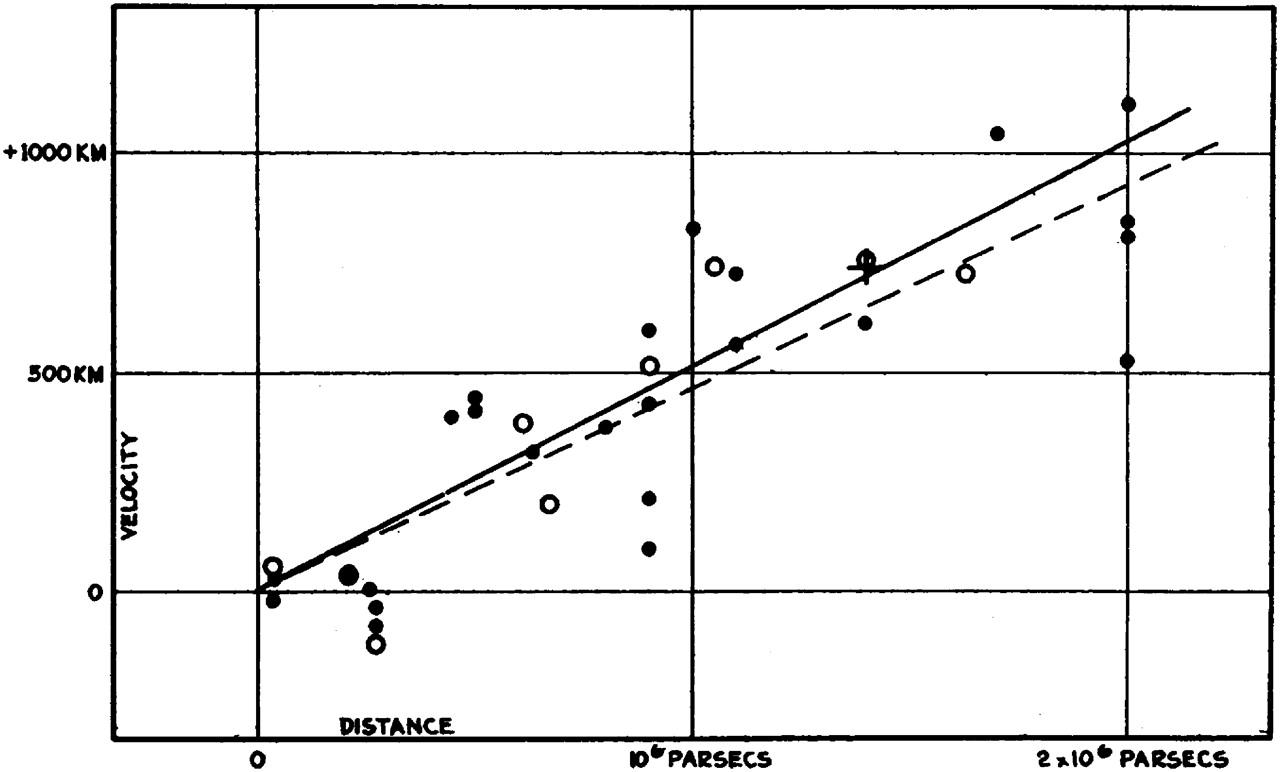
\includegraphics[width=0.75\textwidth]{../figures/01_cosmology/Hubble.jpg}
  \caption[Figure originale d'Edwin Hubble de la vitesse d'éloignement
  de galaxies en fonction de leur distance.]{Figure originale d'Edwin
    Hubble \citep{Hubble1929} de la vitesse d'éloignement en km.s$^{-1}$
  de galaxies en fonction de leur distance en parsecs.}
\label{fig:hubble}
\end{figure}


\subsection{\'Equations de Friedmann-Lemaître}

En joignant la métrique FLRW (eq~\ref{eq:FLRW}) et le tenseur
$T_{\mu\nu}$ (eq~\ref{eq:Tmunusimple}) aux équations d'Einstein, nous
obtenons les équations de Friedmann-Lemaître \citep{Friedmann1922}:

\begin{equation}
  \label{eq:Friedmann1}
  H^{2}\triangleq\left(\frac{\dot{a}}{a}\right)^{2}=\frac{8\pi
    G}{3}\rho-\frac{kc^{2}}{a^{2}}+\frac{\Lambda c^{2}}{3}
\end{equation}
\begin{equation}
  \label{eq:Friedmann2}
  \dot{H}+H^{2}=\frac{\ddot{a}}{a}=-\frac{4\pi
    G}{3}(\rho+\frac{3p}{c^{2}})+\frac{\Lambda c^{2}}{3}
\end{equation}
Comme nous pouvons le voir avec le taux d'expansion, ces équations
décrivent l'évolution temporelle du facteur d'échelle en fonction du
contenu de l'Univers.

En combinant les deux équations de Friedmann, nous pouvons déterminer
l'évolution de la densité du fluide, décrite par son équation de
conservation:

\begin{equation}
  \label{eq:conservationdensity}
  \rho \dot{a} = -\frac{p}{c^{2}}\frac{\d a^{3}}{\d t} \Longrightarrow
  \dot{\rho}=-3H(\rho+\frac{p}{c^{2}})
\end{equation}

En supposant l'équation d'état d'un fluide parfait tel que $p=w(a)\rho
c^{2}$, on obtient que:

\begin{equation}
  \label{eq:30}
  \rho=\rho_{0}f(a)
\end{equation}
avec
\begin{equation}
  \label{eq:31}
  f(a)=\exp{-3\int_{a_{0}}^{a}\frac{1+w(a)}{a}\d a}
\end{equation}
où $a$ correspond au facteur d'échelle à un temps $t$. Si on suppose que
le paramètre $w$ est constant, alors la densité d'un fluide évolue avec
le facteur d'échelle comme:
\begin{equation}
  \label{eq:rhoevol}
  \rho=\rho_{0}\left(\frac{a}{a_{0}}\right)^{-3(1+w)}
\end{equation}

Nous pouvons considérer trois types de fluides cosmologiques modélisant
le contenus dans notre
Univers, pour lesquels la valeur de $w$ va différer:
\begin{itemize}
\item Les fluides composés de particules non-relativistes, comme la
  matière baryonique et la matière sombre. Pour cette composante, on
  considère que sa densité est entièrement décrite par son énergie de
  masse, la pression exercée est donc
  nulle et sa densité se dilue avec le volume uniquement: $\rho_{M}\propto a^{-3}$. L'équation d'état pour la matière vaut $w_{M}=0$;
\item Les fluides composés de particules relativistes, comme les
  photons ou les neutrinos. Ce fluide va se diluer d'une part comme
  de la matière non-relativiste avec le volume ($\propto a^{-3}$), mais également en
  subissant un étirement de longueur d'onde avec le facteur d'échelle
  ($\propto a^{-1}$). La dilution de densité est donc
  $\rho_{R}\propto a^{-4}$ pour ce type de fluide, et son équation d'état est de
  $w_{R}=\frac{1}{3}$;
\item Enfin pour une constante cosmologique $\Lambda$, sa densité est
  par définition constante avec le temps, et $\rho_{\Lambda}\propto
  a^{0}$. Ce fluide a donc une pression négative et ne se dilue pas
  avec le facteur d'échelle, et son équation d'état vaut $w_{\Lambda}=-1$.
\end{itemize}

Nous pouvons introduire pour chaque fluide la densité réduite et
adimensionnées, définit comme le
rapport entre la densité du fluide et la densité dite critique
$\rho_{c}\triangleq\frac{3H^{2}}{8\pi G}$ (à
laquelle l'Univers est nécessairement plat) tel que:
\begin{equation}
  \label{eq:33}
  \Omega_{X}\triangleq\frac{\rho_{X}}{\rho_{c}}
\end{equation}

La première équation de Friedmann-Lemaître peut ainsi se réécrire
simplement comme:
\begin{equation}
  \label{eq:friedmannOmega}
  H^{2}=H_{0}^{2}\left[\Omega_{R,0}\left(\frac{a_{0}}{a}\right)^{4}
    +\Omega_{M,0}\left(\frac{a_{0}}{a}\right)^{3} +\Omega_{k,0}\left(\frac{a_{0}}{a}\right)^{2}+\Omega_{\Lambda,0} \right]
\end{equation}
et en utilisant la définition du redshift:
\begin{equation}
  \label{eq:friedmannZ}
  H^{2}=H_{0}^{2}\left[\Omega_{R,0}(1+z)^{4}
    +\Omega_{M,0}(1+z)^{3} +\Omega_{k,0}(1+z)^{2}+\Omega_{\Lambda,0} \right]
\end{equation}
avec:
\begin{align*}
  \Omega_{X,0}&=\frac{8\pi G}{3H_{0}^{2}}\rho_{X,0} \text{ pour
  $X\in$\{$R$;$M$\}}\\
  \Omega_{k,0}&=-\frac{kc^{2}}{a_{0}^{2}H_{0}^{2}}\\
  \Omega_{\Lambda,0}&=\frac{\Lambda c^{2}}{3H_{0}^{2}}
\end{align*}

Par construction, les paramètres de densité réduite sont reliés par
$\sum_{i\ne k}\Omega_{i}=1-\Omega_{k}$.
L'équation \ref{eq:friedmannOmega} nous montre ainsi que l'évolution de
l'expansion de l'Univers est décrit par 4 paramètres indépendants:
$\Omega_{R}$, $\Omega_{M}$, $\Omega_{\Lambda}$ et $H_{0}$; $\Omega_{k}$
étant contraint par les autres $\Omega_{i}$ et nous renseignant
directement sur la géométrie de l'Univers. Les paramètres $\Omega_{i}$
sont de ce fait appelés \textit{paramètres cosmologiques}. On notera
que, du fait de 
la dégénerescence entre les densités réduites et la constante de Hubble,
il est généralement plus adéquat de mesurer directement la quantité
$\Omega_{i}h^{2}$, où $h=H/100$ km.s$^{-1}$.Mpc$^{-1}$.

\subsection{Mesures de distances}

\subsubsection*{Distance comobile}
La distance comobile caractérise la distance entre deux objets
de telle sorte qu'elle soit indépendante de l'expansion de
l'Univers.

Considérons le voyage d'un photon entre le moment d'émission $t=t_{e}$
à un redshift $z=z_{e}$, et sa réception aujourd'hui à $t=t_{0}$ et
$z=z_{0}=0$. Ce photon se déplacera le long d'une géodésique nulle ($\d
s^{2}=0$), et l'équation \ref{eq:FLRW2} nous donne ainsi (pour $\theta$
et $\phi$ constants) que:

\begin{equation}
  \label{eq:distcomobil}
  d_{c}(z)\triangleq\chi(z)=\int^{t_{0}}_{t_{e}}\frac{c}{a(t')}\d
  t'=\frac{c}{H_{0}}\int_{z=0}^{z=z_{e}}\frac{\d z'}{E(z')}
\end{equation}
avec $E(z)=H^{2}(z)/H_{0}^{2}$, définie par la première équation de
Friedmann comme (eq~\ref{eq:friedmannZ}):
\begin{equation}
  \label{eq:Ez}
  E(z)^{2}=\frac{H^{2}(z)}{H_{0}^{2}}=\Omega_{R,0}(1+z)^{4}
  +\Omega_{M,0}(1+z)^{3} +\Omega_{k,0}(1+z)^{2}+\Omega_{\Lambda,0}
\end{equation}

\subsubsection*{Distance de diamètre angulaire}

La distance de diamètre angulaire $d_{a}$ est définie comme le rapport entre le
diamètre physique $D$ d'un objet et sa taille angulaire apparente
$\Delta\theta$ par:
\begin{equation}
  \label{eq:angulardist1}
  d_{a}=\frac{D}{\Delta\theta}
\end{equation}
Or, d'après la métrique FLRW (eq~\ref{eq:FLRW2}), un objet situé à une
distance comobile $\chi$ à un temps $t$ et avec un angle apparent
$\Delta\theta$ à une taille de:
\begin{equation}
  \label{eq:tailleangulardist}
  D = a(t)S_{k}(\chi)\Delta\theta
\end{equation}
et donc, la distance angulaire s'exprime comme:
\begin{equation}
  \label{eq:angulardist2}
  d_{a}=a(t)S_{k}(\chi)
\end{equation}

Avec le changement de variable $k\rightarrow
-\frac{a_{0}^{2}H_{0}^{2}\Omega_{k,0}}{c^{2}}$, nous obtenons que:
\begin{equation}
  \label{eq:43}
  S_{k}(\chi) = \frac{c}{a_{0}H_{0}\sqrt{\lvert\Omega_{k,0}\rvert}}S_{k}\left(\frac{a_{0}H_{0}\sqrt{\lvert\Omega_{k,0}\rvert}}{c}\chi(z)\right)
\end{equation}

Et ainsi, avec la définition de $\chi$ (eq~\ref{eq:distcomobil}), la
distance de diamètre angulaire s'écrit:

\begin{equation}
  \label{eq:distangulargen}
  d_{a}(z)=\frac{1}{1+z}\frac{c}{H_{0}\sqrt{\lvert\Omega_{k,0}\rvert}}S_{k}\left(\sqrt{\lvert\Omega_{k,0}\rvert}\int_{0}^{z}\frac{\d z'}{E(z')}\right)
\end{equation}

Dans le cas d'un univers plat ($k=0$ et $S_{k}(\chi)=\chi$), nous
pouvons déduire immédiatement la relation:
\begin{equation}
  \label{eq:angulardistflat}
  d_{a}(z)=\frac{d_{c}(z)}{1+z}
\end{equation}


\subsubsection*{Distance de luminosité}

La distance de luminosité $d_{L}$ est la quantité reliant la luminosité
intrinsèque d'une source et le flux reçu par un observateur à cette
distance $d_{L}$. Cette relation décrit la dilution géométrique du flux
avec le carré de la distance, telle que:
\begin{equation}
  \label{eq:45}
  f=\frac{L}{4\pi D_{L}^{2}}
\end{equation}

En utilisant la forme de $S_{k}(\chi)$ définie dans l'eq~\ref{eq:43},
nous pouvons direcement déterminer la surface $S$ d'une sphére centrée
sur la source étudiée à la distance comobile $\chi$:
\begin{equation}
  \label{eq:spheredistlum}
  S=4\pi
  a_{0}^{2}\frac{c^{2}}{a_{0}^{2}H_{0}^{2}\Omega_{k,0}}S_{k}\left( \frac{a_{0}H_{0}\sqrt{\lvert\Omega_{k,0}\rvert}}{c}\chi(z)\right)
\end{equation}

Un photon émis à un temps $t$ est reçu par l'observateur à $t=t_{0}$
avec une énergie diluée d'un facteur ($1+z$). Par ailleurs, deux photons
successifs sont reçus dans un intervalle de temps lui aussi dilaté
d'un facteur ($1+z$). La luminosité propre de la source étudiée dans le
référentiel de l'observateur $L'$ est par conséquent diluée d'un facteur
$(1+z)^{2}$. Le flux surfacique reçu, $f=L'/S$, s'exprime ainsi:
\begin{equation}
  \label{eq:47}
  f=\frac{L}{4\pi
  a_{0}^{2}\frac{c^{2}}{a_{0}^{2}H_{0}^{2}\Omega_{k,0}}S_{k}\left( \frac{a_{0}H_{0}\sqrt{\lvert\Omega_{k,0}\rvert}}{c}\chi(z)\right)}\times\frac{1}{(1+z)^{2}}
\end{equation}

En utilisant la relation de la dilution géométrique du flux
(\ref{eq:45}) et l'expression de $\chi$ (\ref{eq:distcomobil}), on
obtiens finalement la forme de la distance de luminosité:
\begin{equation}
  \label{eq:48}
  d_{L}(z) = \frac{c(1+z)}{H_{0}\sqrt{\lvert\Omega_{k,0}\rvert}}S_{k}\left(\sqrt{\lvert\Omega_{k,0}\rvert}\int_{0}^{z}\frac{\d z'}{E(z')}\right)
\end{equation}

Nous pouvons noter que, quelque soit la courbure de l'Univers,
$d_{L}(z)=(1+z)^{2}d_{a}(z)$. Dans le cadre d'un Univers plat, la
distance de luminosité est reliée à la distance comobile par
$d_{L}(z)=(1+z)\chi(z)=(1+z)d_{c}(z)$.

\subsubsection*{Le module de distance}
Comme illustré dans l'équation\ref{eq:48}, la distance de luminosité
permet de contraindre les paramètres cosmologiques. Afin de remonter à
cette information, il est nécessaire de connaître la luminosité
intrinsèque de la source observée.

On définit dans un premier temps la magnitude apparente $m$ d'un objet
observé par:
\begin{equation}
  \label{eq:magapp}
  m-m_{0}=-2.5\log_{10}\left(\frac{f}{f_{0}}\right) = -2.5\log_{10}\left(\frac{L}{L_{0}}\frac{d_{L,0}^{2}}{d_{L}^{2}}\right)
\end{equation}
avec $f$ le flux lumineux apparent de la source, et $m_{0}$ la magnitude
apparente (connue) d'un objet de flux $f_{0}$ (connu) utilisé comme
point zéro.

On introduit la magnitude absolue $M$ de l'objet, défini comme étant
sa magnitude si l'objet était situé à une distance de $d_{L,0}=10$
pc. Cette quantité est ainsi associée à la luminosité intrinsèque de la
source observée. Le module de distance est alors défini comme étant:
\begin{equation}
  \label{eq:distmodulemu}
  \mu\triangleq m-M=5\log_{10}\left(\frac{d_{L}}{10\text{pc}}\right)
\end{equation}
\section{Sondes cosmologiques et modèle de concordance \lcdm}\label{ssec:LCDM}

L'étude de la relativé générale aux échelles cosmologiques, de
l'expansion de l'Univers ou encore de sa composation nécéssite
l'utilisation d'observables, appelées \textit{sondes cosmologiques}.
Les différents modèles cosmologiques et leurs prédictions sont ensuite
testés par ses observations. L'utilisation de plusieurs sondes
indépendantes permet
par ailleurs de lever de potentielles dégénerescences entre les paramètres
cosmologiques, et ainsi contraindre fortement les différents modèles
existants.

Nous présentons ici brièvement les principales sondes cosmologiques
utilisées, et comment leur utilisation a permis de converger vers le
modèle standard de la cosmologie moderne, le modèle \lcdm, décrivant un
Univers plat ($k=0$) avec une constante cosmologique $\Lambda$.

\subsection{Le fond diffus cosmologique}

Comme nous l'avons abordé avec le principe cosmologique, le rayonnement
du fond diffus cosmologique est une source primordiale d'information sur
notre Univers. Prédit par Lemaître en 1920 et découvert en 1965 par
\citet{Penzias1965}, ce rayonnement est une véritable relique de notre
Univers, s'agissant du plus ancien rayonnement électromagnétique
observable ($z\sim 1100$). Initialement à une température de l'ordre de
$3000K$, l'expansion de l'Univers a considérablement dilué l'énergie des
photons du CMB, amenant sa température actuelle à
$T_{0}=2.7260\pm0.0013K$ \citep{Fixsen2009}. Les
premières études des fluctuations de température du CMB, faites avec les missions COBE et WMAP, ont
permis de confirmer que son spectre est celui d'un corps noir
quasi-parfait. Les mesures les plus récentes du CMB ont été effectuées avec la mission
Planck.
Le spectre de puissance\footnote{transformée
de Fourier de la fonction de corrélation à deux points} des anisotropies
de ce rayonnement est prédictible par les modèles cosmologiques, et
permet d'en contraindre fortement les paramètres. La
Figure~\ref{fig:cmbTTplanck} présente l'ajustement du modèle standard
\lcdm\ avec le spectre de puissance des fluctuations de température du
CMB \citep{Planckparams2018}.

\begin{figure}[ht]
  \begin{minipage}[c]{0.55\textwidth}
    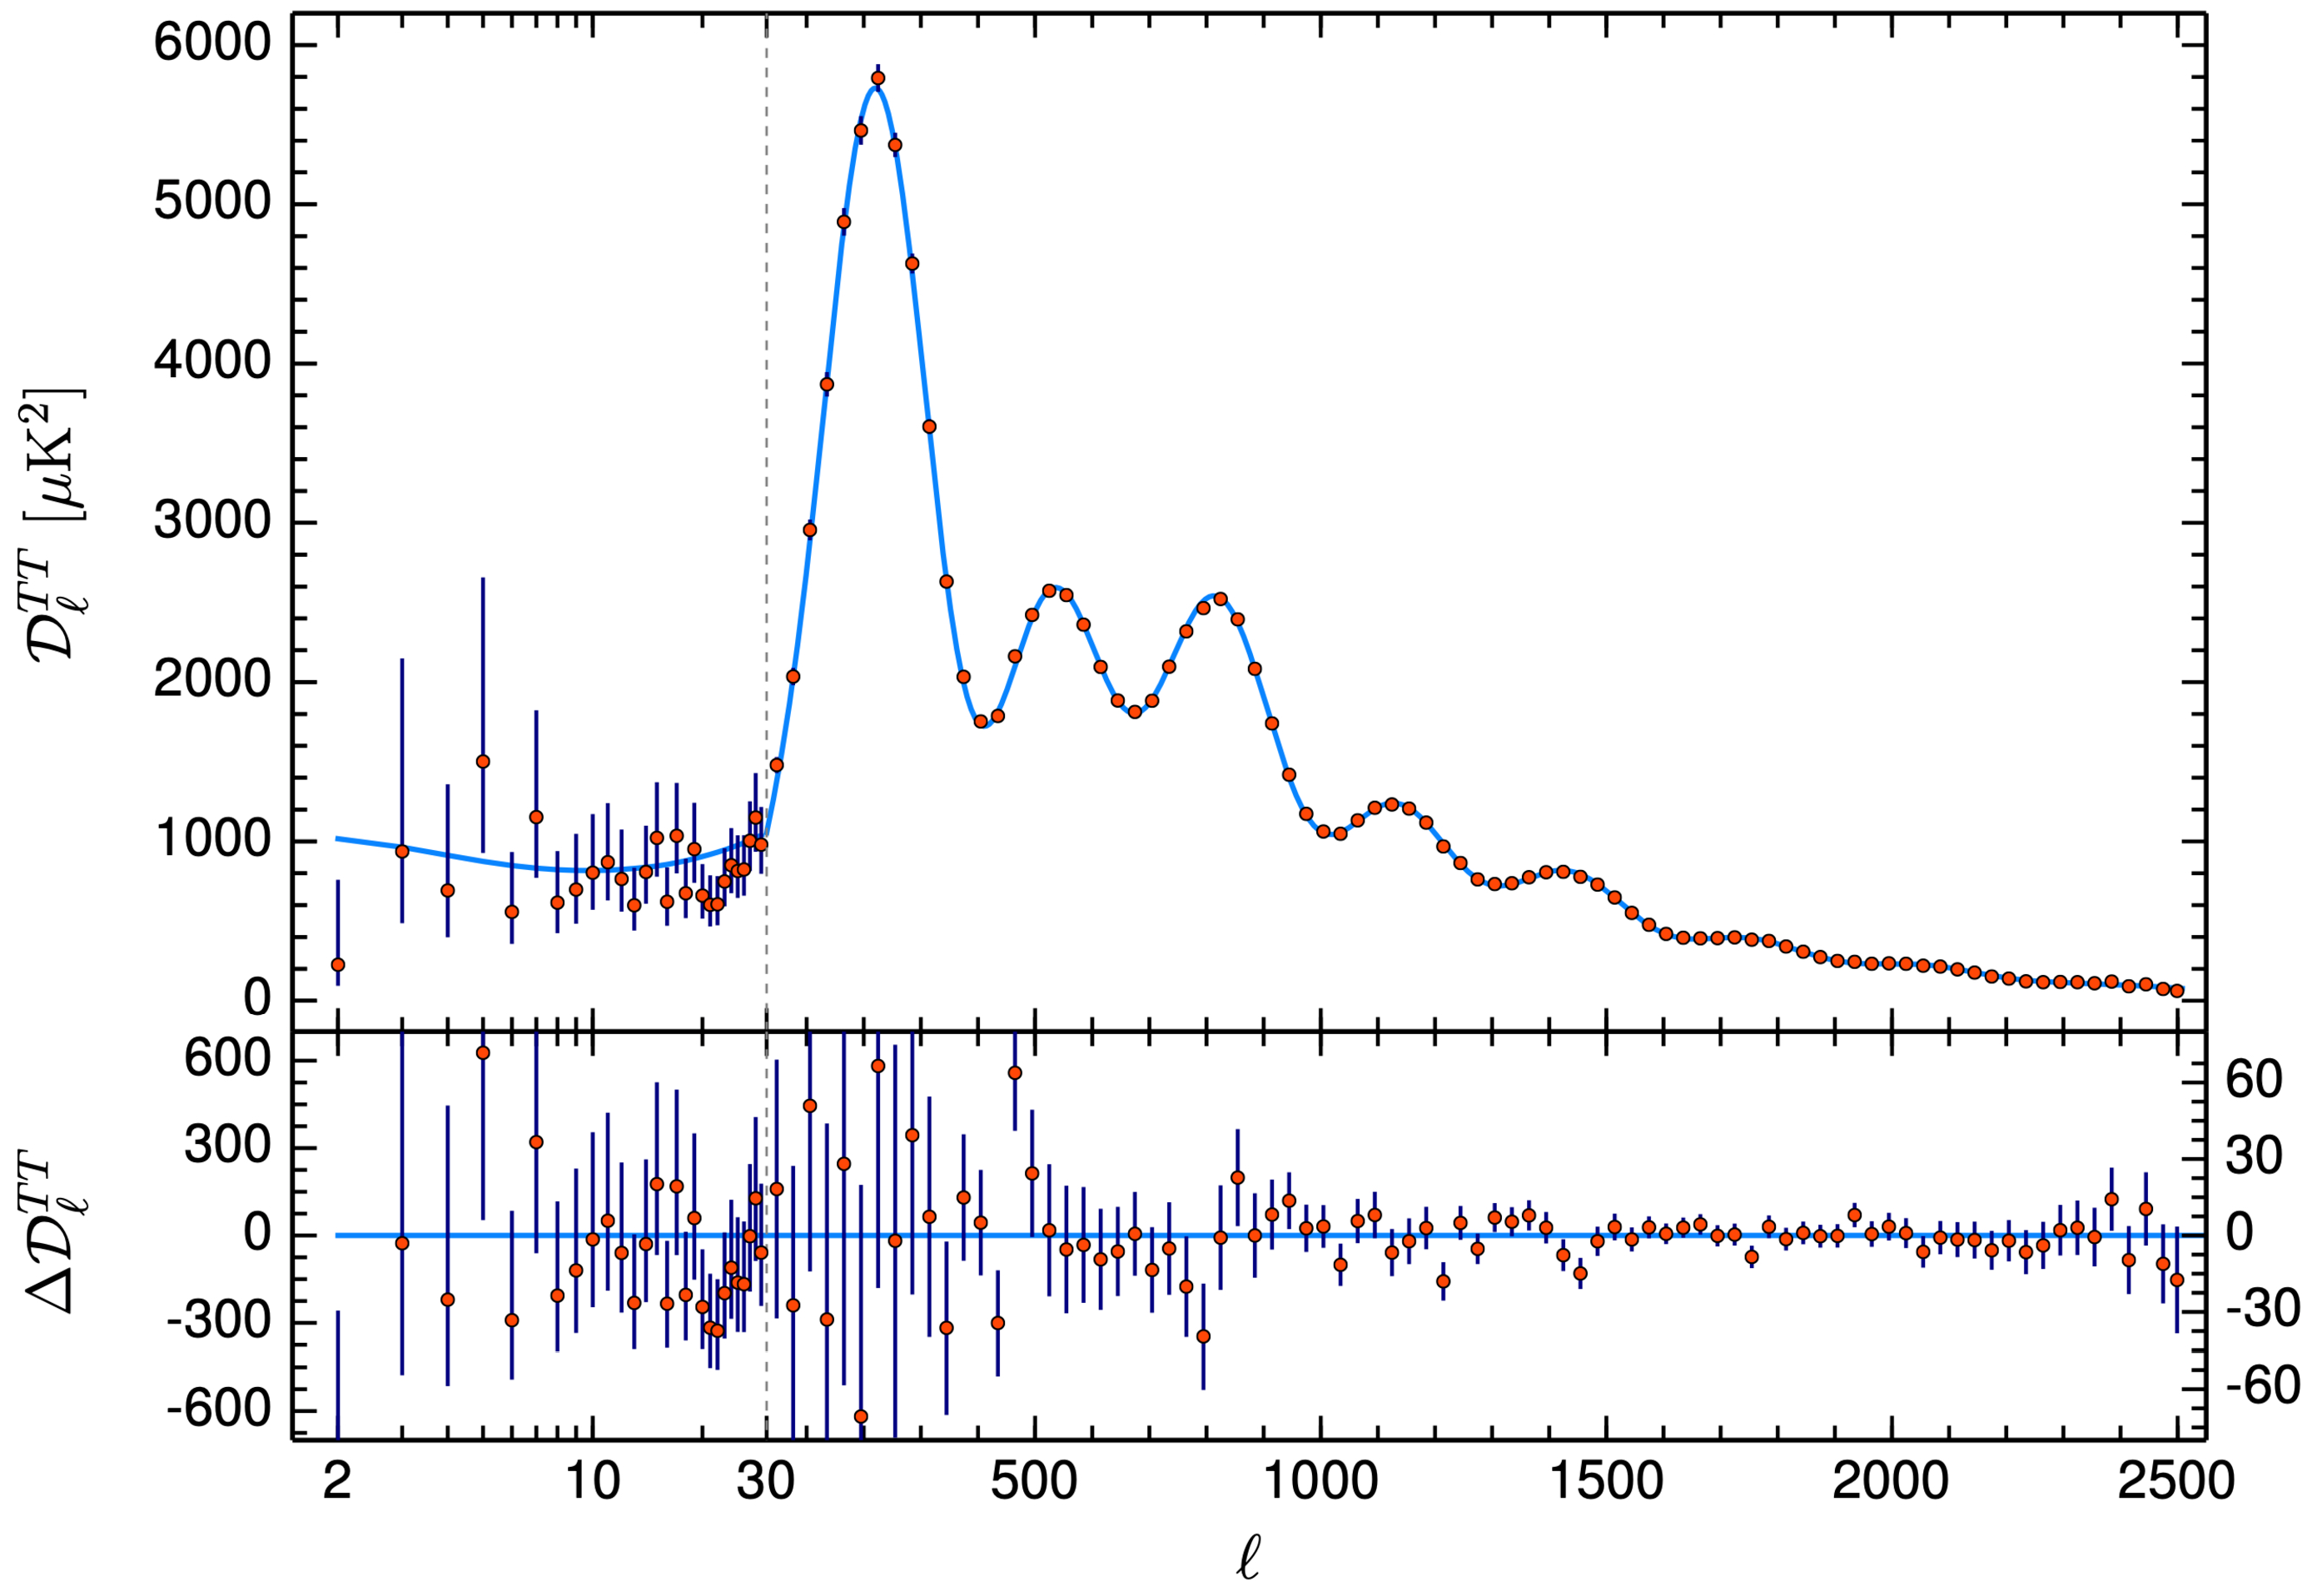
\includegraphics[width=\textwidth]{../figures/01_cosmology/cmbTTplanck.pdf}
  \end{minipage}\hfill
  \begin{minipage}[c]{0.44\textwidth}
    \caption[Spectre de puissance des anisotropies en température du
    CMB.]{Spectre de puissance des anisotropies en température du
    CMB. L'axe des abscisses représente le multipôle, où les grandes
    échelles angulaires correspondent à un petit $l$ et inversement. Les
    points rouges représentent les données, et la courbe bleu le
    meilleur ajustement du modèle \lcdm. En bas sont illustrés les
    résidus entre le modèle et les données. Figure de \citet{Planckparams2018}.}\label{fig:cmbTTplanck}
  \end{minipage}
\end{figure}

\subsection{Les oscillations acoustiques des baryons}

Les oscillations acoustiques des baryons, une autre sonde cosmologique,
correspondent à un phénomène trouvant sa source bien avant le découplage entre la
matière baryonique et les photons. Au moment de l'inflation (phase
d'expansion exponentielle de l'Univers $\sim10^{-35}s$ le Big Bang), des
fluctuations de densité se sont propagées dans le plasma composant l'Univers
primordial. Alors que les zones de surdensités ainsi créées attirent
gravitationnellement la matière vers elles, la pression radiative des
photons contre cet effet, créant des oscillations acoustiques sphériques
dans l'Univers primordial.

Au moment de la recombinaison, les intéractions entre photons et baryons cessent,
et les photons sont libres de voyager à la vitesse de la lumière. L'onde acoustique ne se
propage plus et laisse ainsi une zone de surdensité à une distance
caractéristique. Cette distance est celle 
parcourue par l'onde entre sa création ($z=\infty$) et la
recombinaison ($z\sim1100$), appelée horizon sonore. Ce pic de densité est ainsi figé
depuis le découplage baryon/photon. L'Univers étant en expansion, la
taille caractéristique de cette empreinte est exprimée en distance
comobile, et vaut $r_{d}\sim105$ Mpc.h$^{-1}$.
En relevant le redshift de plus d'un million de galaxie entre $0<z<0.6$
et en étudiant leur fonction de corrélation à deux points,
le relevé SDSS \citep{YorkSDSS2000} a permis de mesurer pour la première fois le pic du BAO
en 2005 \citep[Figure~\ref{fig:baopeak};][]{Eisenstein}. Ce pic traduit ainsi un excès de probabilité d'observer 2 galaxies
séparées par une distance $r_{d}$, signature caractéristique des ondes
acoustiques primordiales. 


\begin{figure}[ht]
  
  \begin{minipage}[c]{0.42\textwidth}
    \caption[Mise en évidence du pic de BAO avec le relevé SDSS.]{Mise en
      évidence du pic de BAO avec le relevé SDSS. Cette figure de
      \citet{Eisenstein} montre la fonction de corrélation à deux points
      des galaxies du relevé SDSS. Le pic à environ $105$ Mpc.h$^{-1}$ est
      clairement visible, et caractérise le pic des BAO. Les lignes vertes,
      rouges et bleues correspondent au modèle de concordance \lcdm\, que
      nous introduirons plus tard, pour différentes valeurs de
      $\Omega_{M,0}h^{2}$. La ligne magenta correspond à un modèle sans
      constante cosmologique.}\label{fig:baopeak}
    \end{minipage}
    \begin{minipage}[c]{0.55\textwidth}
      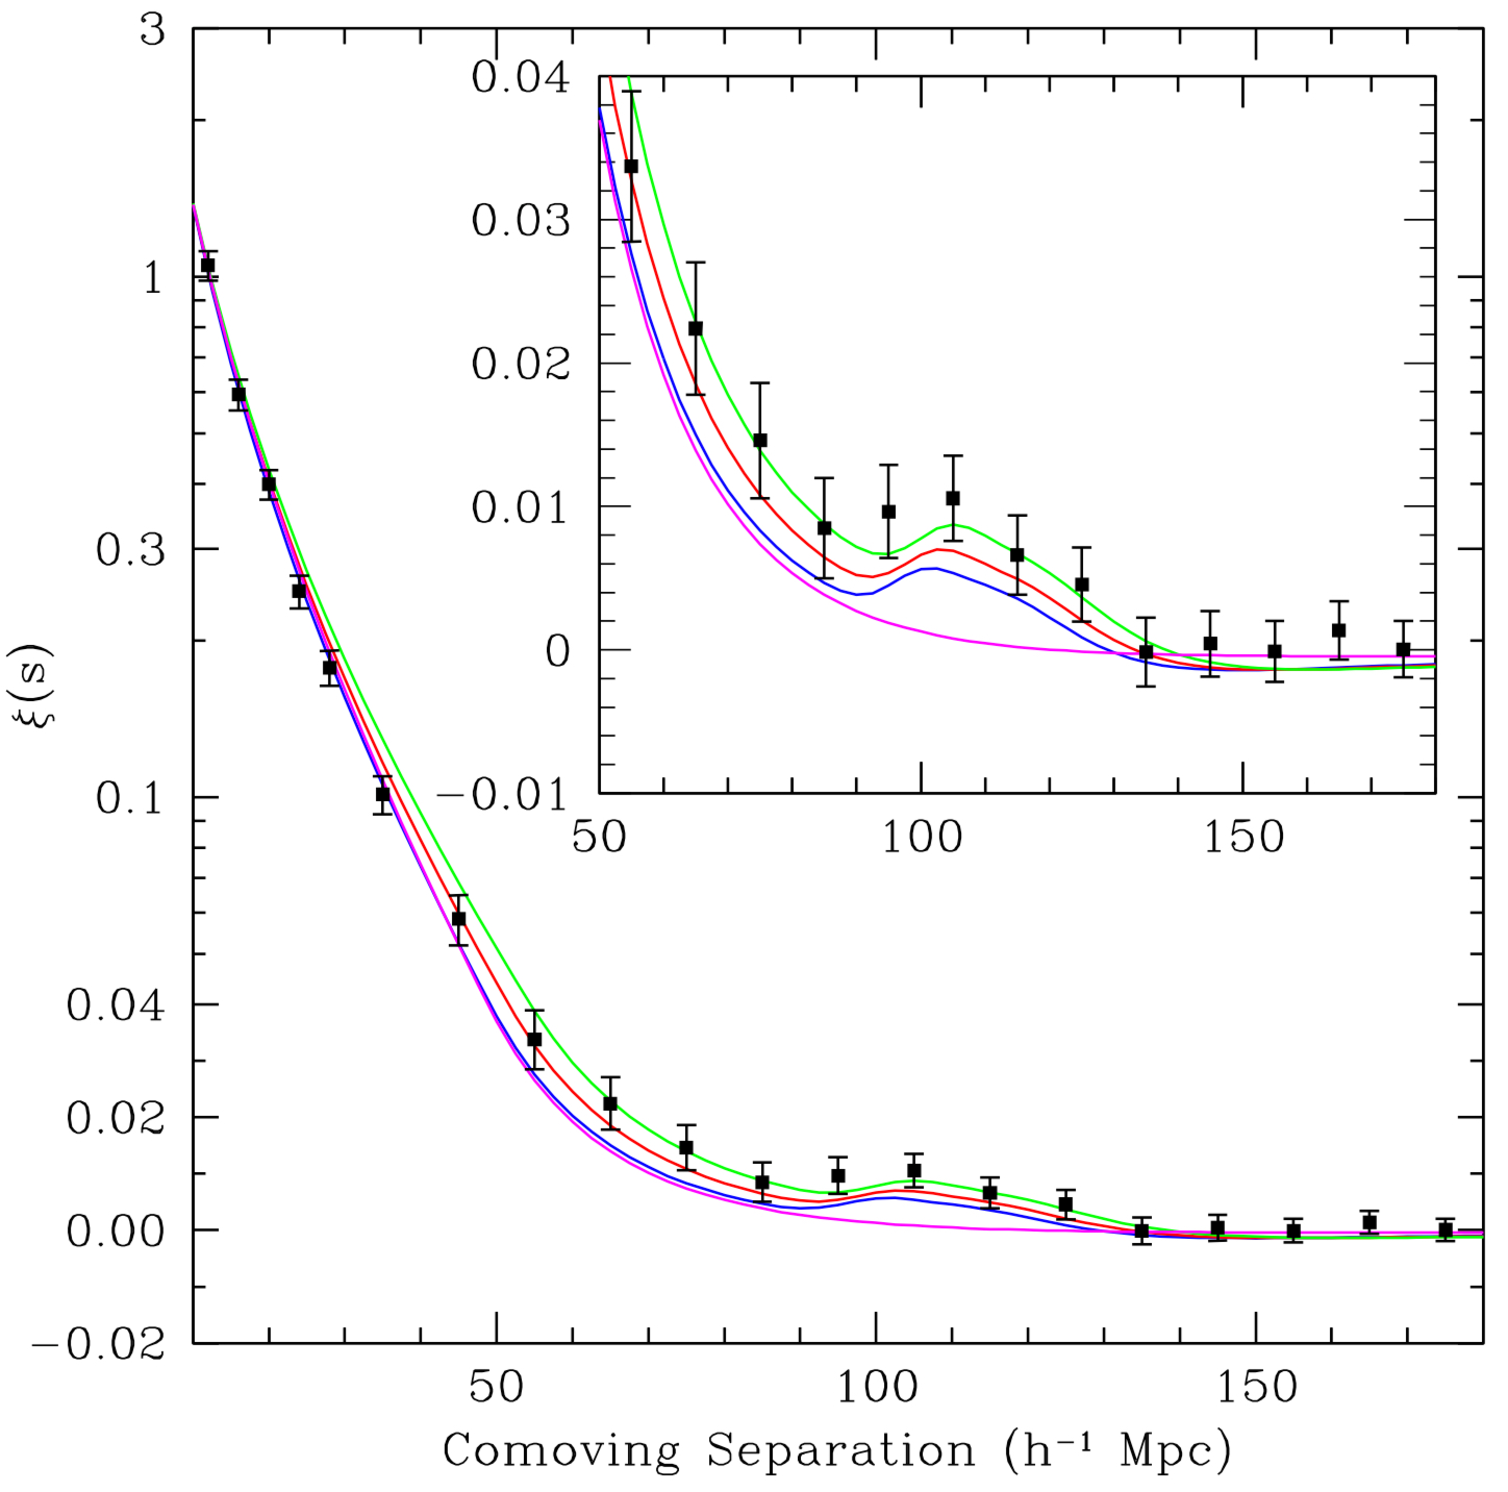
\includegraphics[width=\textwidth]{../figures/01_cosmology/BAOpeak.pdf}
    \end{minipage}\hfill
  
\end{figure}

La distance caractéristique $r_{d}$ est scindée
entre sa composante transverse $r_{\parallel}$ et radiale $r_{\perp}$,
tels que:
\begin{align}
  \label{eq:bao}
  r_{\parallel}&=\frac{c\Delta z}{H(z)}\\
  r_{\perp}&=d_{c}(\bar{z})\theta
\end{align}
où $\Delta z$ et $\theta$ sont l'intervalle en redshift et
l'angle sur lesquelles s'étendent l'échelle caractéristique des
BAO. $d_{c}$ représente la distance comobile, que l'on peut déduire
directement de la métrique FLRW et qui dépend des paramètres
cosmologiques. La mesure des BAO permettent ainsi d'ajuster une
cosmologie aux données, et par conséquent de sonder l'évolution du taux
d'expansion avec le redshift et de
contraindre les paramètres cosmologiques.

\subsection{Les chandelles standard}

Comme nous l'avons vu avec la dérivation des différentes distances
cosmologiques, la distance de luminosité permet de contraindre les
paramètres cosmologiques. Obtenir cette information nécessite cependant
de connaître \textit{a
  priori} la luminosité intrisèque de l'objet étudié.

Si cette luminosité absolue est reproductible, alors la source
astronomique est qualifiée de chandelle standard. La mesure de sa
luminosité apparente permet alors de remonter à sa distance de luminosité, et apporter des
contraintes sur les paramètres cosmologiques. 

Les supernovae de type Ia (SNeIa), classification particulière d'explosion
d'étoile, sont un exemple de chandelle standard ayant permis la
découverte de l'accélération de l'expansion de l'Univers
\citep{Riess1998, Perlmutter1999}.

La courbe de lumière des SNeIa (évolution de leur luminosité au cours du
temps), est fortement caractéristique, permettant par une méthode de
standardisation de remonter à leur luminosité intrinsèque. Nous montrons
dans la Figure~\ref{fig:sneiabetoule} l'évolution des distances ainsi dérivées d'un échantillon de SNeIa en
fonction de leur redshift. Le modèle ajusté aux données correpond au
modèle standard de la cosmologie, le modèle \lcdm.

\begin{figure}[ht]
  \begin{minipage}[c]{0.55\textwidth}
    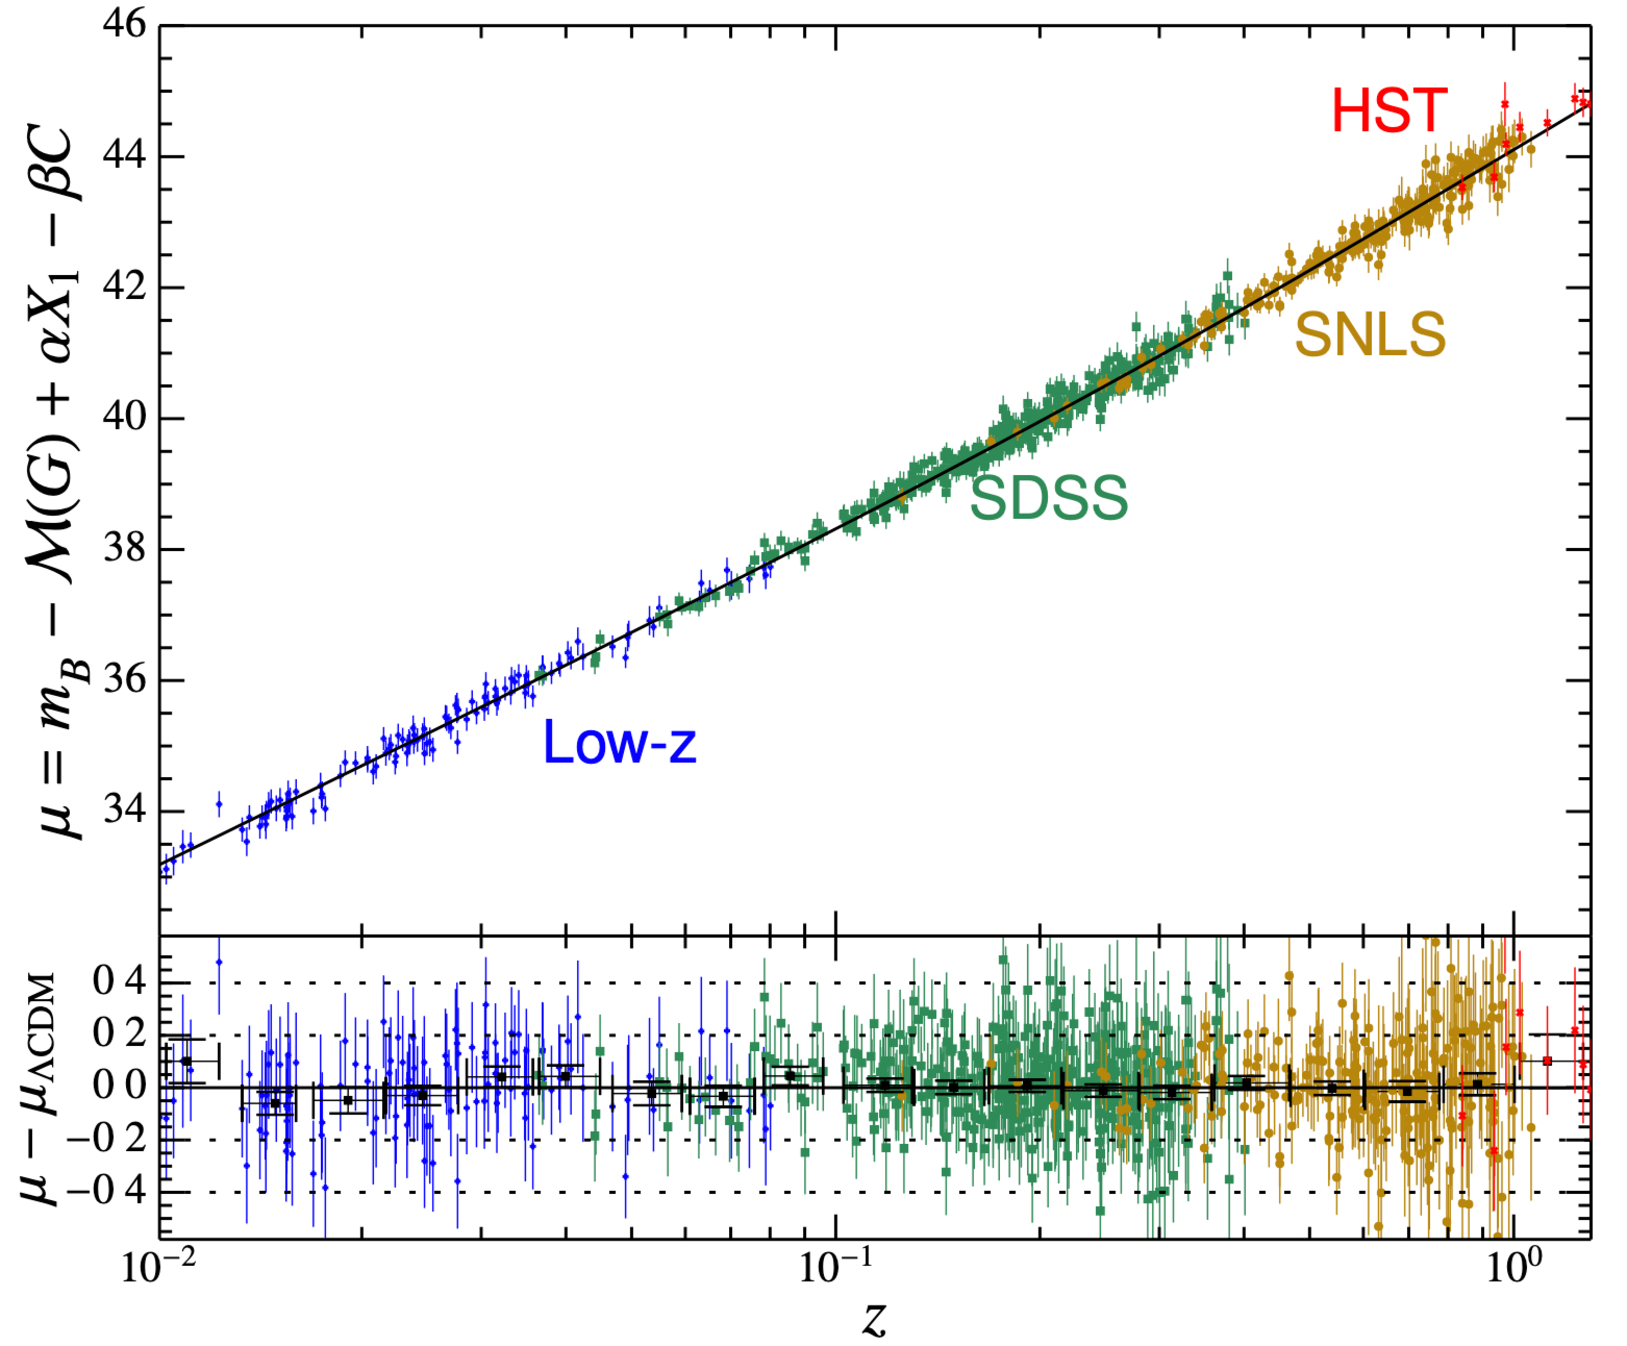
\includegraphics[width=\textwidth]{../figures/01_cosmology/sneiabetoule.pdf}
  \end{minipage}\hfill
  \begin{minipage}[c]{0.42\textwidth}
    \caption[Diagramme de Hubble à partir de SNeIa de plusieurs relevés
    (SDSS, SNLS, HST)]{Diagramme de Hubble à partir de 740 SNeIa de plusieurs relevés
    (SDSS, SNLS, HST). La partie haute de cette figure montre
    l'évolution du module de distance en fonction du redshift
  des SNeIa de l'échantillon. La courbe noire correspond au modèle
  cosmologique \lcdm\ ajusté aux données. La partie du bas montre les résidus entre
  les données et le modèle \lcdm. Figure de \citet{Betoule2014}.}\label{fig:sneiabetoule}
  \end{minipage}
\end{figure}

Ces objets étant au coeur de ce travail de recherche, nous leur dédions une
partie plus loin dans ce chapitre. 


\subsection{Le modèle \lcdm}
L'étude de ces nombreuses sondes indépendantes combinées (comme le fond diffus
cosmologique, les oscillations acoustiques des baryons, les supernovae
de type Ia, etc) permettent de converger vers un modèle unique: le
modèle de concordance. Ce modèle cosmologique décrit un Univers plat
($k=0$), rempli de radiation, de  matière
baryonique (à hauteur de $6\%$), de matière sombre froide ($26\%$)
et d'énergie sombre sous la forme d'une constante cosmologique
($68\%$).

La radiation, dominante aux premiers âges de l'Univers, est aujourd'hui
négligeable, sa densité évoluant en $\propto a^{-4}$. La matière baryonique désigne celle que nous
connaissons, composée de baryons comme les protons et les neutrons. La
matière sombre est une matière hypothétique, détectée indirectement par
ses effets gravitationnelles et pouvant expliquer les propriétés
observées des galaxies ou amas de galaxies (masses, vitesses de
rotation etc). Elle est qualifiée de \textit{sombre} car elle n'intéragirait que
très faiblement avec la matière ordinaire et le champ
électromagnétique, et de \textit{froide} pour décrire une vitesse de
déplacement faible par rapport à celle de la lumière. La constante
cosmologique permet d'expliquer l'accélération de l'expansion de
l'Univers découverte à la fin du XX\ieme\ siècle.

Ce modèle, appelé \lcdm\ (\textit{Lambda Cold Dark Matter}) en
référence aux deux composantes exotiques décrites plus tôt,
correspond au modèle standard de la cosmologie moderne. On notera que
malgré la prédiction de ces composantes sombre, le modèle \lcdm\ ne
précise en aucun cas leur nature, encore inconnue à ce jour.

Composé de seulement six paramètres libres, le modèle de concordance
rend compte de nombreuses observations cosmologiques comme le fond
diffus cosmologique, les structures à grandes échelles de la
distribution des galaxies, l'expansion accélérée de l'Univers,
l'abondance des éléments légers (hydrogène, hélium, lithium) etc.

Les derniers résultats d'ajustement de ces paramètres libres du modèle \lcdm\ sur les
observations (sondes cosmologiques) ont été présentés
par la collaboration Planck \citep{Planckparams2018}. Il est également
possible de tester le modèle \lcdm\ en laissant libre certains
paramètres contraints ou fixés \textit{a priori} comme l'équation d'état
de l'énergie sombre ($w=-1$) ou la composante de courbure
($\Omega_{k}=0$).
Nous montrons dans la Figure~\ref{fig:flatcontrainte} les contraintes dans le plan
($\Omega_{M}$,$\Omega_{\Lambda}$) et dans le plan ($\Omega_{k}$,$\Omega_{M}$), en utilisant une combinaison de
sondes cosmologiques, permettant de réduire considérablement la
dégénerescence entre les paramètres. Cette analyse effectuée en laissant
la courbure libre dans l'ajustement des paramètres de \lcdm\ (dénommé o-\lcdm), fait clairement état
de la compatibilité des données observationnelles avec un Univers
plat. Cette contrainte sur la courbure de l'Univers est principalement
apportée par le fond diffus cosmologique. 

\begin{figure}[ht]
\centering
\subfloat[]{\label{fig:omegamomegal}{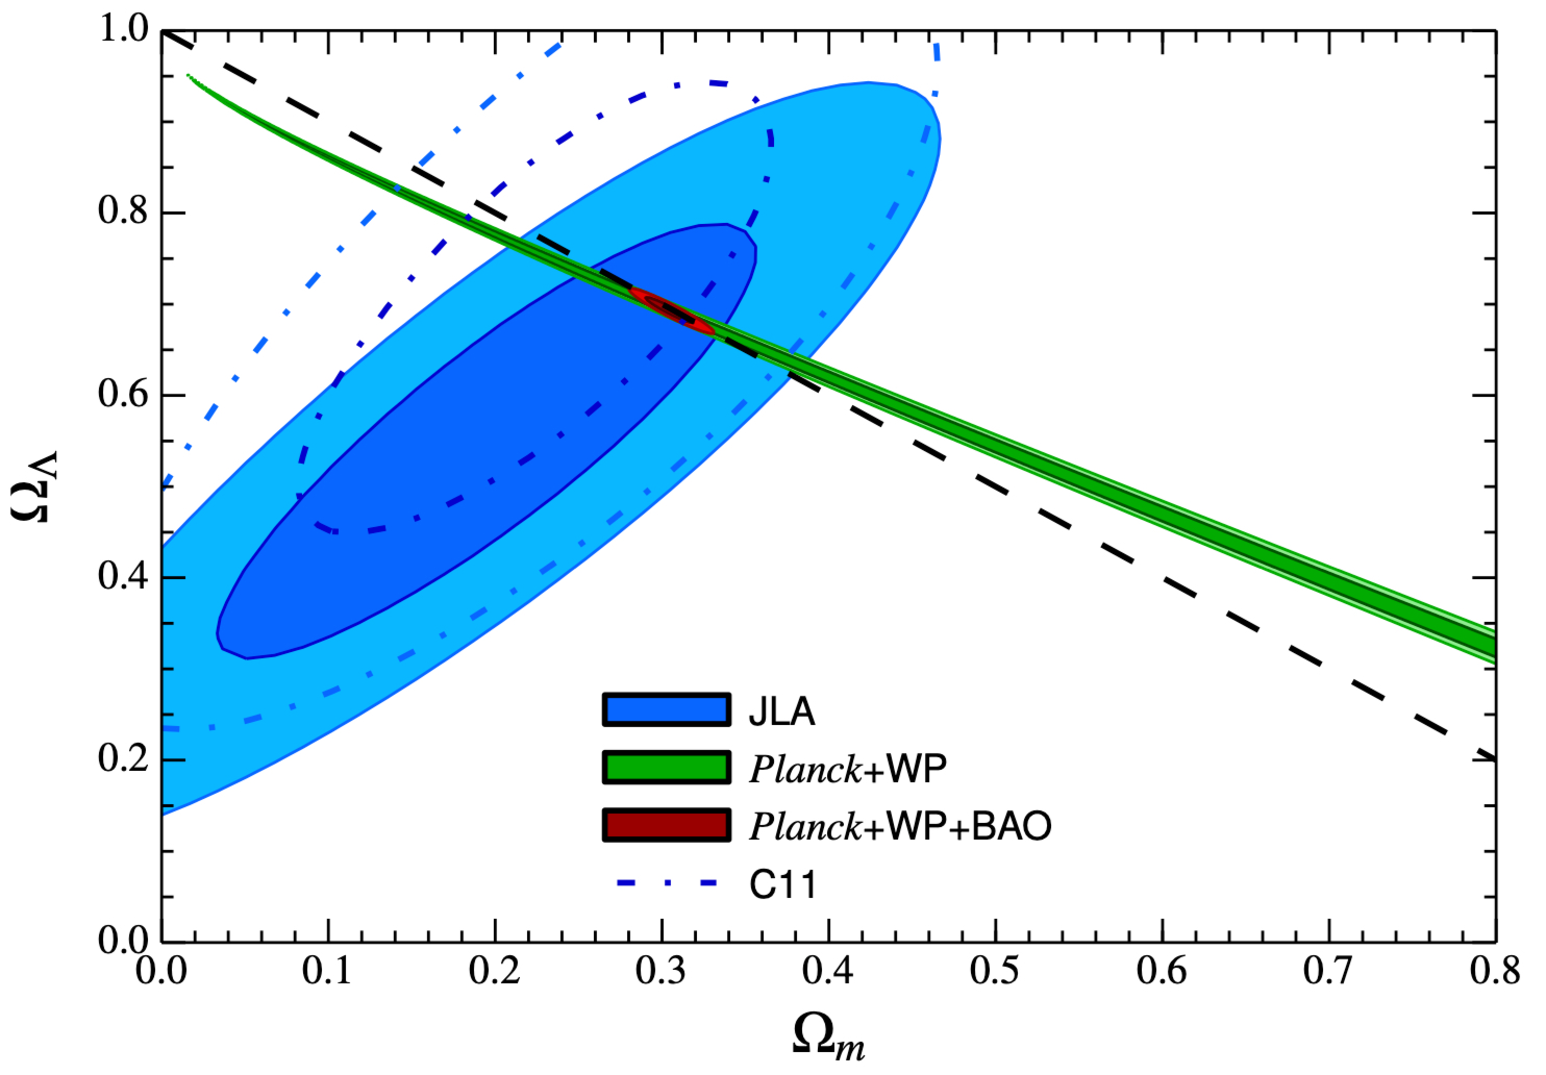
\includegraphics[width=0.5\textwidth]{../figures/01_cosmology/Betoule_omegaM_omega_L.pdf}}}\hfill
\subfloat[]{\label{fig:omegakomegam}{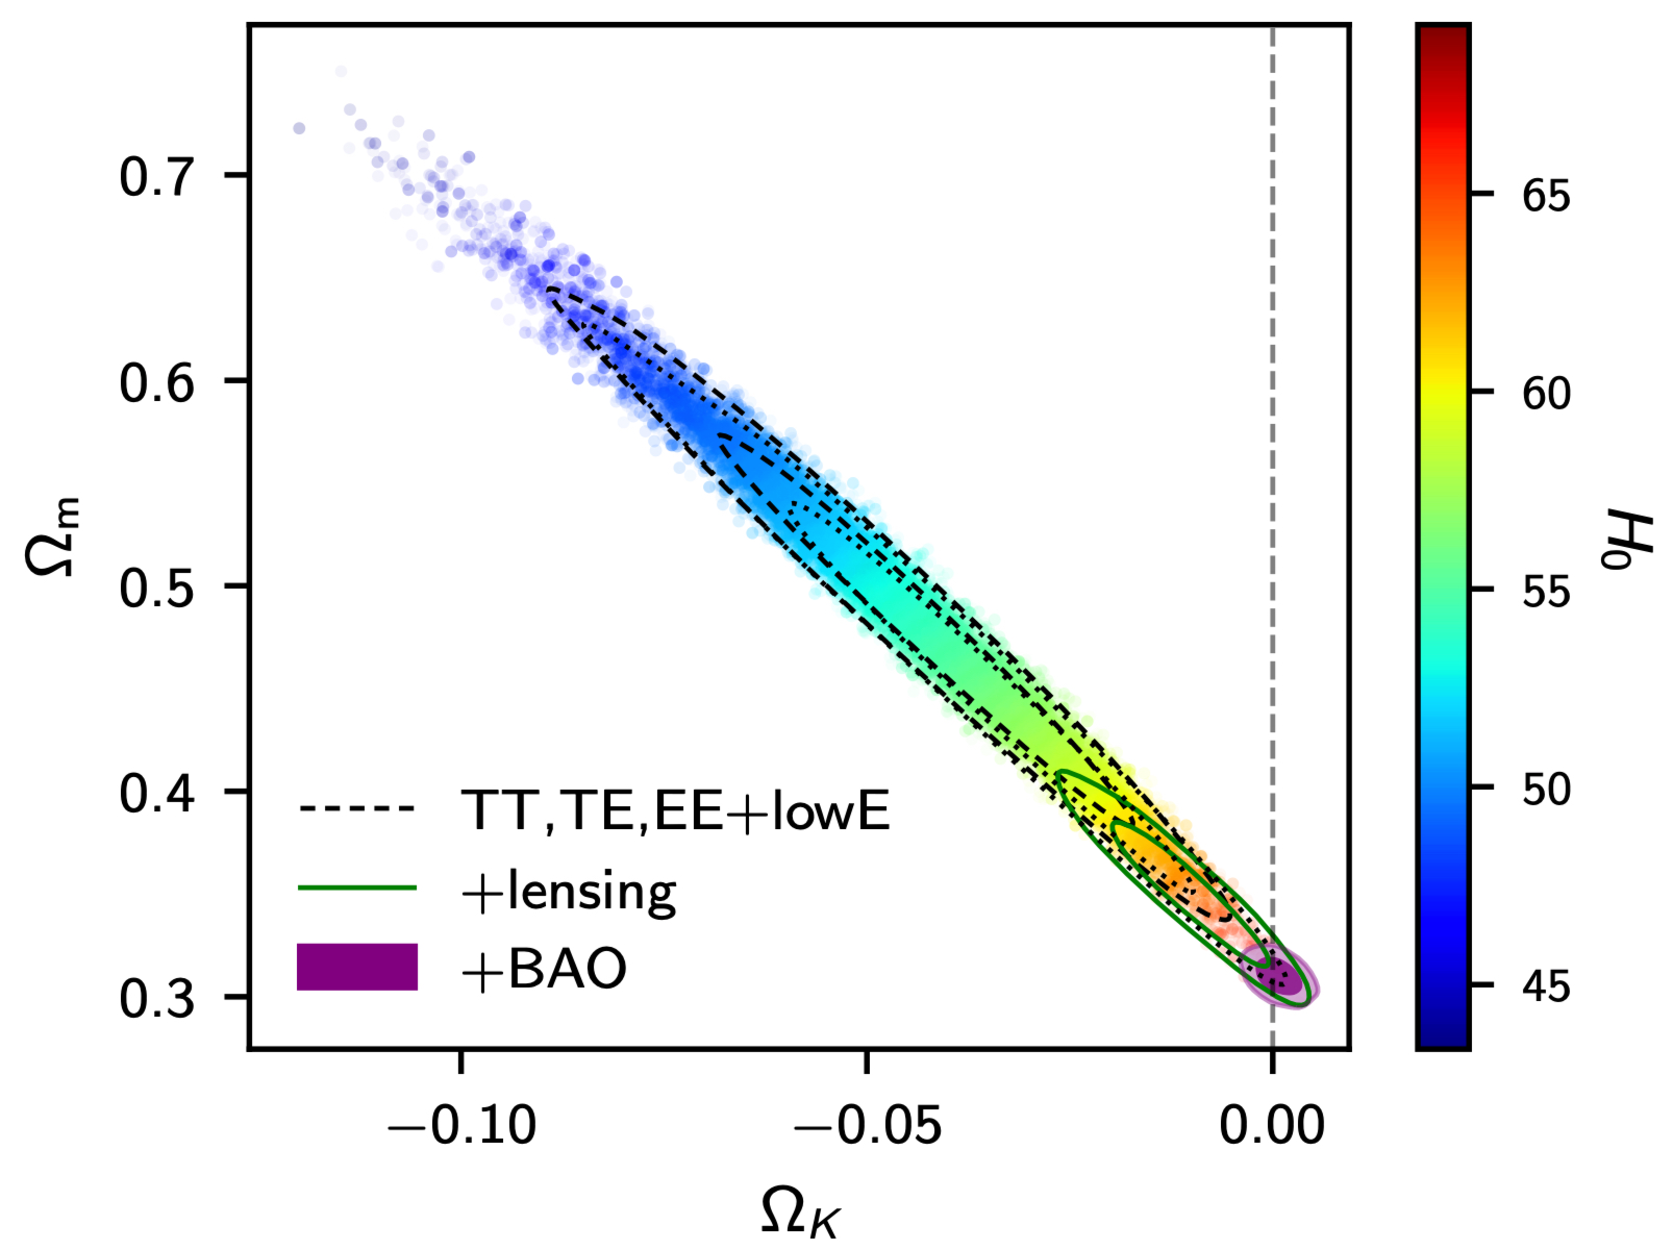
\includegraphics[width=0.5\textwidth]{../figures/01_cosmology/PlanckOmegakOmegam.pdf}}}
\caption[]{(a) Contraintes dans le plan
  ($\Omega_{M}$,$\Omega_{\Lambda}$) en combinant les sondes
  cosmologiques de supernovae de type Ia \citep[JLA,][]{Betoule2014}, du
  CMB (Planck+WP 2014) et d'oscillation
  acoustique des baryons (BAO). Figure de\citet{Betoule2014}. (c)
  Contraintes dans le plan ($\Omega_{k}$,$\Omega_{M}$) en utilisant le
  CMB et son lentillage gravitationnelle, et les BAO. Figure de \citet{Planckparams2018}.}
\label{fig:flatcontrainte}
\end{figure}

De la même manière, l'hypothèse de constante cosmologique peut être
testée en laissant le paramètre d'équation d'état $w_{DE}$ de l'énergie
sombre libre (modèle $w$-\lcdm). Pour aller encore plus loin, il est
également possible de sonder une potentielle caractéristique dynamique
de la densité de l'énergie sombre, en paramétrisant $w_{DE}$ par:
\begin{equation}
  \label{eq:wCPL}
  w(a)=w_{0}+w_{a}(1-a)
\end{equation}
aussi appelée paramétrisation CPL \citep{CPL2001,Linder2003}. Ainsi, si
l'énergie sombre est en effet une constante cosmologique dans les
équations d'Einstein, alors $w_{0}=-1$ et $w_{a}=0$. La
Figure~\ref{fig:darkenergy} illustre les contraintes récentes,
compatibles avec le modèle \lcdm, sur le
paramètre $w$ et sur les composantes de la paramétrisation CPL $w_{0}$
et $w_{a}$.
Les contraintes cosmologiques sur $w$
sont dérivées de mesures de variations relatives de distance de
luminosité en fonction du redshift. Les propriétés de chandelle standard
des SNeIa en font ainsi une sonde cosmologique prafaitement adaptée à l'étude
de l'énergie sombre.

\begin{figure}[ht]
\centering
\subfloat[]{\label{fig:womegam}{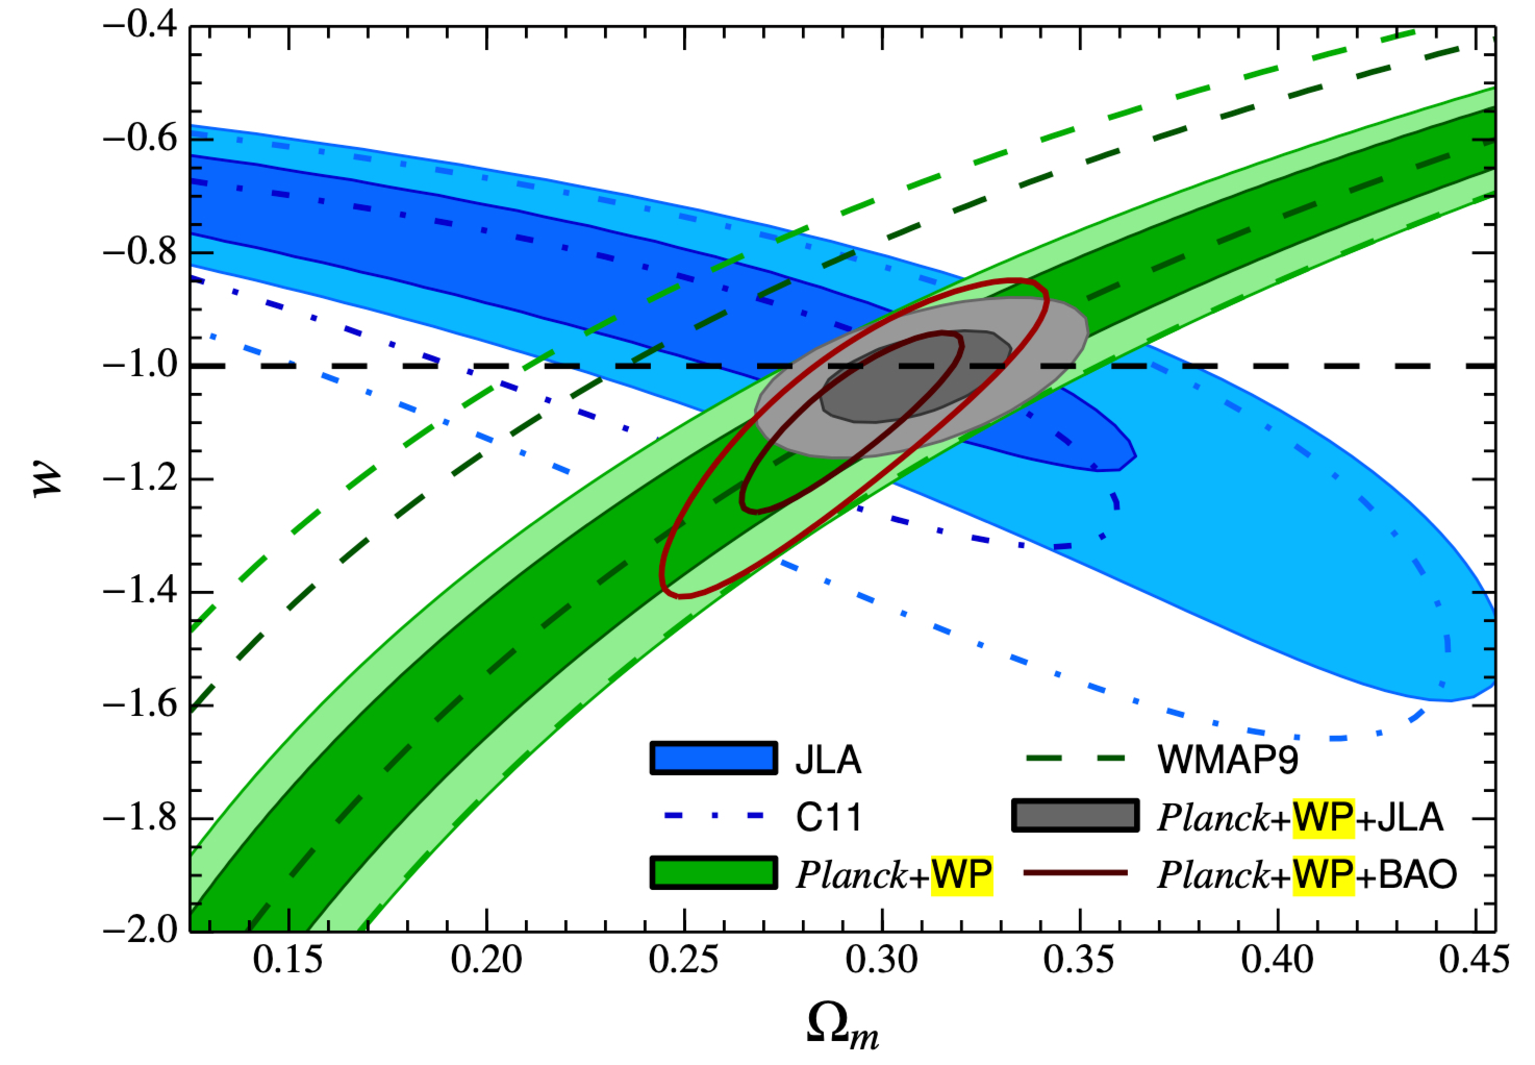
\includegraphics[width=0.5\textwidth]{../figures/01_cosmology/BetoulewomegaM.pdf}}}\hfill
\subfloat[]{\label{fig:w0wa}{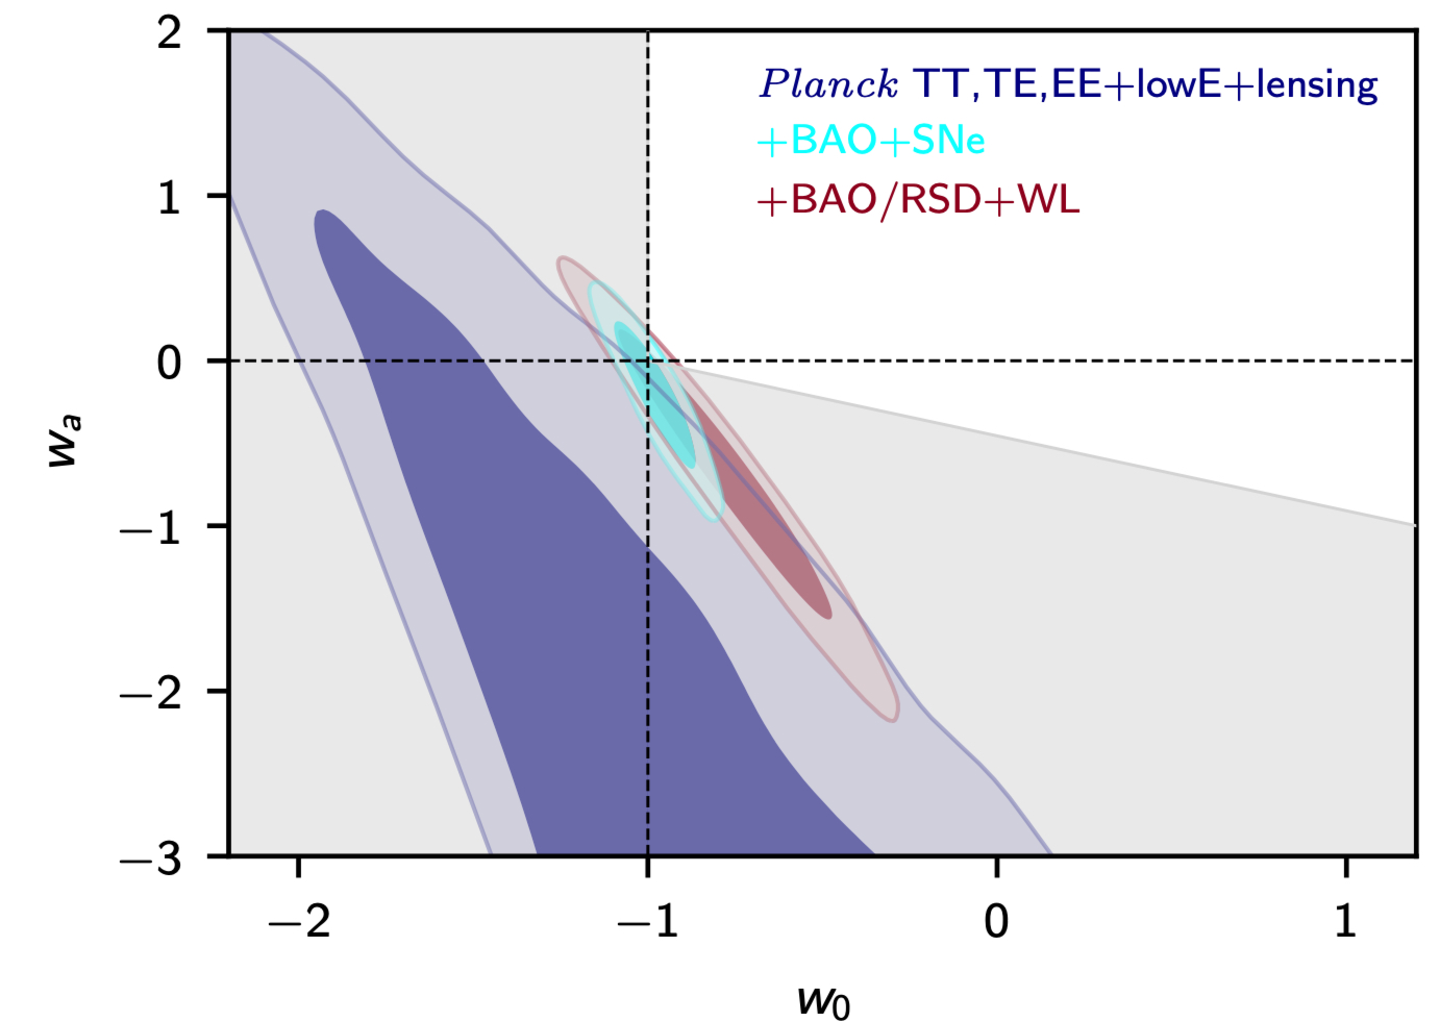
\includegraphics[width=0.5\textwidth]{../figures/01_cosmology/Planckw0wa.pdf}}}
\caption[]{(a) Contraintes dans le plan
  ($w$,$\Omega_{M}$) en combinant les sondes
  cosmologiques de supernovae de type Ia \citep[JLA,][]{Betoule2014}, du CMB (Planck+WP 2014) et d'oscillation
  acoustique des baryons (BAO). Figure de \citet{Betoule2014}. (c)
  Contraintes dans le plan ($w_{a}$,$w_{0}$) en utilisant le
  CMB et son lentillage gravitationnelle, les supernovae de Pantheon
  \citep{Scolnicpantheon18} et les BAO. Figure de \citet{Planckparams2018}.}
\label{fig:darkenergy}
\end{figure}

%\bibliographystyle{../main/aa_url2}
%\bibliography{99_references}
\end{document}

%%% Local Variables:
%%% mode: latex
%%% TeX-master: t
%%% End:
